\documentclass[]{article}
\usepackage[utf8]{inputenc}
\usepackage{graphicx}
\usepackage{array}
\usepackage{amsmath}

\title{Análisis de Mezcla de Combustibles para Optimización de Costos y Reducción de Emisiones}
\author{}
\date{}

\begin{document}
	
	\maketitle
	
	\section*{Introducción}
	El uso de combustibles en la industria y el transporte ha sido fundamental para el desarrollo económico a lo largo de la historia. Sin embargo, el impacto ambiental causado por las emisiones de gases contaminantes y el aumento de los costos energéticos han motivado a las empresas a buscar soluciones más sostenibles y eficientes. La mezcla de diferentes tipos de combustibles, como la gasolina, el diésel y los biocombustibles, se ha convertido en una estrategia prometedora para optimizar el consumo energético y reducir el impacto ambiental.
	
	Este estudio tiene como objetivo analizar cómo la combinación de varios combustibles puede cumplir con objetivos específicos, como minimizar costos, maximizar la eficiencia energética y reducir las emisiones contaminantes. Utilizando un enfoque basado en \textbf{sistemas de ecuaciones lineales}, exploraremos cómo determinar la mezcla óptima de combustibles para alcanzar un equilibrio entre costo, eficiencia y sostenibilidad.
	
	\section*{Desarrollo}
	
	\subsection*{1. Contexto y Problemática}
	Las empresas que dependen del uso intensivo de combustibles, como las compañías de transporte, las fábricas y las plantas de generación de energía, enfrentan desafíos en la gestión de costos operativos y en el cumplimiento de normativas ambientales cada vez más estrictas. El precio de los combustibles fósiles fluctúa de acuerdo con las condiciones del mercado global, mientras que el uso de biocombustibles puede contribuir a reducir las emisiones de dióxido de carbono.
	
	En este escenario, las empresas se enfrentan a la siguiente pregunta: \textbf{¿Cómo pueden combinar diferentes fuentes de energía de manera eficiente para reducir costos y minimizar el impacto ambiental sin sacrificar el rendimiento?}
	
	\subsection*{2. Definición del Problema}
	Supongamos que una empresa de transporte desea utilizar una mezcla de tres tipos de combustibles para abastecer su flota de vehículos:
	
	\begin{itemize}
		\item \textbf{Gasolina} (Combustible A)
		\item \textbf{Diésel} (Combustible B)
		\item \textbf{Biocombustible} (Combustible C)
	\end{itemize}
	
	El objetivo es encontrar la cantidad óptima de cada tipo de combustible para cumplir con los siguientes requisitos:
	\begin{itemize}
		\item \textbf{Contenido energético mínimo}: El vehículo necesita al menos 800 unidades de energía para funcionar de manera óptima.
		\item \textbf{Límite de emisiones de CO2}: Las emisiones no deben exceder las 500 unidades.
		\item \textbf{Minimizar el costo total de la mezcla}: Se tiene un presupuesto limitado.
	\end{itemize}
	
	\subsection*{3. Datos del Problema y Planteamiento de las variables}
	A continuación, se presenta la información relevante sobre los combustibles disponibles:
	
	\begin{center}
		\begin{tabular}{|c|c|c|c|c|}
			\hline
			Propiedad & Gasolina (A) & Diésel (B) & Biocombustible (C) \\
			\hline
			Energía (unidades/Litro) & 10 & 1 & 8 \\
			\hline
			Emisiones de CO2 (unidades/Litro) & 7 & 2 & 2 \\
			\hline
			Costo (\$/Litro) & 3 & 4 & 6 \\
			\hline
		\end{tabular}
	\end{center}
	
	\subsection*{4. Sistema de Ecuaciones}
	Queremos encontrar las cantidades \textbf{x}, \textbf{y} y \textbf{z} que representen la cantidad en litros de gasolina, diésel y biocombustible, respectivamente, que cumplan con las siguientes ecuaciones:
	
	\begin{itemize}
		\item \textbf{1. Contenido energético mínimo:} 10x + 1y + 8z $\geq$ 800
		\item \textbf{2. Límite de emisiones de CO2:} 7x + 2y + 2z $\leq$ 500
		\item \textbf{3. Minimizar el costo total:} Costo = 3x + 4y + 6z
	\end{itemize}
	
	\subsection*{5. Sistema de Ecuaciones Lineales}
	Convertimos las restricciones en un sistema de ecuaciones lineales para simplificar el análisis y resolverlo. El sistema es el siguiente:
	
	\[ 
	\begin{cases}
		10x + 1y + 8z = 800 \\
		7x + 2y + 2z = 500 \\
		3x + 4y + 6z = 600
	\end{cases}
	\]
	
	El sistema puede representarse mediante la matriz aumentada:
	
	\[
	\begin{bmatrix}
		10 & 1 & 8 & | & 800 \\
		7 & 2 & 2 & | & 500 \\
		3 & 4 & 6 & | & 600
	\end{bmatrix}
	\]
	
	\subsection*{6. Resolución del Sistema con el Método de la Matriz Inversa}
	Para resolver el sistema utilizando el método de la matriz inversa, planteamos el sistema de ecuaciones de la siguiente manera:
	
	\[
	\begin{bmatrix}
		10 & 1 & 8 \\
		7 & 2 & 2 \\
		3 & 4 & 6
	\end{bmatrix}
	\begin{bmatrix}
		x \\
		y \\
		z
	\end{bmatrix}
	=
	\begin{bmatrix}
		800 \\
		500 \\
		600
	\end{bmatrix}
	\]
	
	Ahora vamos a calcular la matriz inversa de la matriz de coeficientes:
	
	\[
	\begin{bmatrix}
		10 & 1 & 8 \\
		7 & 2 & 2 \\
		3 & 4 & 6
	\end{bmatrix}
	\]
	
	\subsubsection*{Paso 1: Cálculo de la matriz inversa}
	La fórmula para la matriz inversa de una matriz 3x3 es:
	
	\[
	A^{-1} = \frac{1}{\text{det}(A)} \cdot \text{adj}(A)
	\]
	
	donde \(\text{det}(A)\) es el determinante de la matriz \(A\) y \(\text{adj}(A)\) es la matriz adjunta de \(A\).
	
	Primero, calculamos el determinante de la matriz \(A\):
	
	\[
	\text{det}(A) = 10 \cdot (2 \cdot 6 - 4 \cdot 2) - 1 \cdot (7 \cdot 6 - 3 \cdot 2) + 8 \cdot (7 \cdot 4 - 3 \cdot 5)
	\]
	
	\[
	\text{det}(A) = 10 \cdot (12 - 8) - 1 \cdot (42 - 6) + 8 \cdot (28 - 15)
	\]
	
	\[
	\text{det}(A) = 10 \cdot 4 - 1 \cdot 36 + 8 \cdot 13
	\]
	
	\[
	\text{det}(A) = 40 - 36 + 104 = 108
	\]
	
	
	Ahora, calculamos la matriz adjunta de \(A\). La adjunta de una matriz 3x3 es la transpuesta de la matriz de los cofactores. Los cofactores se calculan como el determinante de las submatrices 2x2 formadas por eliminar la fila y la columna correspondiente a cada elemento de la matriz.
     		
     \begin{figure}[!ht]
     	\centering
     	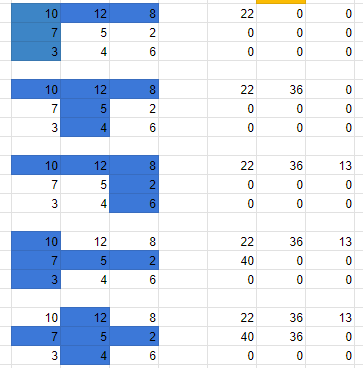
\includegraphics[width=7cm]{adjunta1.png}
     	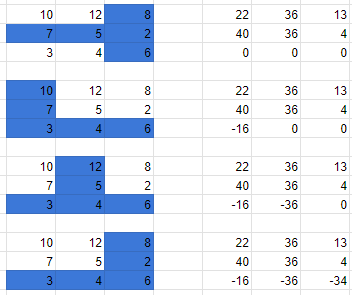
\includegraphics[width=7cm]{adjunta2.png}
     \end{figure}
     
	Finalmente, se multiplica la matriz adjunta por \(\frac{1}{\text{det}(A)}\) para obtener la matriz inversa.
	
	\subsubsection*{Paso 2: Multiplicación de la matriz inversa ya transpuesta por el vector de resultados}
	Una vez que tenemos la matriz inversa, la solución del sistema es:
	\[
	\begin{bmatrix}
		x \\
		y \\
		z
	\end{bmatrix}
	=
	\begin{bmatrix}
		-0.203703703703704 & 0.37037037037037 & 0.148148148148148 \\
		0.333333333333333 & -0.333333333333333 & -0.333333333333333 \\
		-0.12037037037037 & 0.037037037037037 & 0.314814814814815
	\end{bmatrix}
	\begin{bmatrix}
		800 \\
		500 \\
		600
	\end{bmatrix}
	\]
	Realizando la multiplicación de la matriz inversa por el vector de resultados, obtenemos la solución:
	
	\[
	\begin{bmatrix}
		x \\
		y \\
		z
	\end{bmatrix}
	=
	\begin{bmatrix}
		43.333 \\
		60.00 \\
		38.333
	\end{bmatrix}
	\]
	
	Esto confirma que la mezcla óptima es:
	\[
	x = 43.333, \quad y = 60.00, \quad z = 38.333
	\]
	
	\subsection*{7. Resolución del Sistema con el Método de Gauss-Jordan}
	Para resolver el sistema de ecuaciones usando el método de Gauss-Jordan, seguimos los siguientes pasos. Primero, la matriz aumentada es:
	
\[
\begin{bmatrix}
	10 & 1 & 8 & | & 800 \\
	7 & 2 & 2 & | & 500 \\
	3 & 4 & 6 & | & 600
\end{bmatrix}
\]

\section*{Resolución paso a paso}

\subsection*{Paso 1: Normalizar el primer pivote (\(a_{11}\))}

Dividimos la primera fila entre \(10\):

\[
R_1 \rightarrow \frac{R_1}{10}
\]

\[
\begin{bmatrix}
	1 & 0.1 & 0.8 & | & 80 \\
	7 & 2 & 2 & | & 500 \\
	3 & 4 & 6 & | & 600
\end{bmatrix}
\]

\subsection*{Paso 2: Hacer ceros debajo del primer pivote (\(a_{21}\) y \(a_{31}\))}

Usamos \(R_1\) para eliminar los valores en la primera columna de \(R_2\) y \(R_3\):
\[
R_2 \rightarrow R_2 - 7 \cdot R_1
\]
\[
R_3 \rightarrow R_3 - 3 \cdot R_1
\]

El resultado es:

\[
\begin{bmatrix}
	1 & 0.1 & 0.8 & | & 80 \\
	0 & 1.3 & -3.6 & | & -160 \\
	0 & 3.7 & 3.4 & | & 360
\end{bmatrix}
\]

\subsection*{Paso 3: Normalizar el segundo pivote (\(a_{22}\))}

Dividimos la segunda fila entre \(1.3\):

\[
R_2 \rightarrow \frac{R_2}{1.3}
\]

\[
\begin{bmatrix}
	1 & 0.1 & 0.8 & | & 80 \\
	0 & 1 & -2.769 & | & -123.077 \\
	0 & 3.7 & 3.4 & | & 360
\end{bmatrix}
\]

\subsection*{Paso 4: Hacer ceros arriba y abajo del segundo pivote (\(a_{12}\) y \(a_{32}\))}

Usamos \(R_2\) para eliminar los valores en la segunda columna de \(R_1\) y \(R_3\):
\[
R_1 \rightarrow R_1 - 0.1 \cdot R_2
\]
\[
R_3 \rightarrow R_3 - 3.7 \cdot R_2
\]

El resultado es:

\[
\begin{bmatrix}
	1 & 0 & 1.053 & | & 92.308 \\
	0 & 1 & -2.769 & | & -123.077 \\
	0 & 0 & 13.786 & | & 851.538
\end{bmatrix}
\]

\subsection*{Paso 5: Normalizar el tercer pivote (\(a_{33}\))}

Dividimos la tercera fila entre \(13.786\):

\[
R_3 \rightarrow \frac{R_3}{13.786}
\]

\[
\begin{bmatrix}
	1 & 0 & 1.053 & | & 92.308 \\
	0 & 1 & -2.769 & | & -123.077 \\
	0 & 0 & 1 & | & 61.823
\end{bmatrix}
\]

\subsection*{Paso 6: Hacer ceros arriba del tercer pivote (\(a_{13}\) y \(a_{23}\))}

Usamos \(R_3\) para eliminar los valores en la tercera columna de \(R_1\) y \(R_2\):
\[
R_1 \rightarrow R_1 - 1.053 \cdot R_3
\]
\[
R_2 \rightarrow R_2 + 2.769 \cdot R_3
\]

El resultado final es:

\[
\begin{bmatrix}
	1 & 0 & 0 & | & 43.333 \\
	0 & 1 & 0 & | & 60.000 \\
	0 & 0 & 1 & | & 38.333
\end{bmatrix}
\]

\section*{Solución del sistema}

La solución del sistema es:

\[
x = 43.333, \quad y = 60.00, \quad z = 38.333
\]
	
	\subsection*{8. Interpretación de los Resultados}
	La solución nos indica que la mezcla óptima para cumplir con los requisitos de energía y emisiones al menor costo posible es:
	\begin{center}
		\textbf{43.333 litros de Gasolina, 60.00 litros de Diésel, y 38.333 litros de Biocombustible.}
	\end{center}
	
	\section*{Conclusión}
	El análisis de la mezcla de combustibles utilizando un enfoque basado en sistemas de ecuaciones y optimización lineal demuestra ser una herramienta poderosa para las empresas que buscan reducir costos operativos y minimizar su impacto ambiental. Aunque los biocombustibles son generalmente más costosos, su menor nivel de emisiones puede hacerlos más atractivos en escenarios donde las regulaciones ambientales son estrictas.
	
	La implementación de estrategias de mezcla de combustibles no solo permite a las empresas cumplir con las regulaciones, sino que también contribuye a una transición hacia fuentes de energía más sostenibles. Sin embargo, es fundamental realizar análisis detallados y simulaciones para ajustar las proporciones en función de las variaciones en los costos y la disponibilidad de combustibles en el mercado.
	
\end{document}


